\documentclass{article}

\usepackage{fullpage}
\usepackage{amsmath,amsbsy,amsfonts,amssymb,amsthm}
\newtheorem{theorem}{Theorem}


\usepackage{graphicx}
\usepackage{dsfont}
\usepackage{algorithm}
\usepackage{algorithmic}
\usepackage{enumitem}
\usepackage{url}
\usepackage{xcolor}
\usepackage{mdframed}
\usepackage{listings}
\usepackage{minted}
\usepackage{amsmath}


\newcommand{\field}[1]{\mathbb{#1}}
\newcommand{\set}[1]{\mathcal{#1}}
\newcommand{\fY}{\set{Y}}
\newcommand{\fX}{\set{X}}
\newcommand{\fF}{\set{F}}
\newcommand{\fH}{\set{H}}
\newcommand{\fD}{\set{D}}

\newcommand{\R}{\field{R}}
\newcommand{\Nat}{\field{N}}

\renewcommand{\Pr}{\field{P}}
\newcommand{\Ind}{\mathds{1}}
\newcommand{\E}{\field{E}}
\newcommand{\Var}{\mathrm{Var}}

\DeclareMathOperator*{\argmin}{arg\,min}
\DeclareMathOperator*{\argmax}{arg\,max}

\DeclareMathOperator{\sign}{sign}

\newcommand{\RiskD}{L_{\fD}}
\newcommand{\RiskS}{L_{S}}
\newcommand{\RiskSi}{L_{S_i}}
\newcommand{\RiskV}{L_{V}}
\newcommand{\RiskT}{L_{T}}

\newcommand{\blambda}{\boldsymbol{\lambda}}
\newcommand{\bnu}{\boldsymbol{\nu}}
\newcommand{\btheta}{\boldsymbol{\theta}}
\newcommand{\bx}{\boldsymbol{x}}
\newcommand{\bX}{\boldsymbol{X}}
\newcommand{\bw}{\boldsymbol{w}}
\newcommand{\bu}{\boldsymbol{u}}
\newcommand{\bv}{\boldsymbol{v}}
\newcommand{\by}{\boldsymbol{y}}
\newcommand{\bz}{\boldsymbol{z}}
\newcommand{\bV}{\boldsymbol{V}}
\newcommand{\bD}{\boldsymbol{D}}
\newcommand{\bphi}{\boldsymbol{\phi}}
\newcommand{\bPhi}{\boldsymbol{\Phi}}
\newcommand{\bxi}{\boldsymbol{\xi}}
\newcommand{\bbeta}{\boldsymbol{\beta}}
\newcommand{\balpha}{\boldsymbol{\alpha}}

\newcommand{\newdef}[1]{\textbf{#1}}

\newcommand{\norm}[1]{\left\lVert#1\right\rVert}

\DeclareMathOperator{\Conv}{conv}
\newcommand\braces[1]{\{#1\}}
\newcommand\brackets[1]{[#1]}
\newcommand\dotp[1]{\langle #1 \rangle}
\newcommand\Parens[1]{\mleft(#1\mright)}
\newcommand\Norm[1]{\mleft\|#1\mright\|}
\newcommand\Braces[1]{\mleft\{#1\mright\}}
\newcommand\Brackets[1]{\mleft[#1\mright]}
\newcommand\Ceil[1]{\mleft\lceil#1\mright\rceil}
\newcommand\Abs[1]{\mleft|#1\mright|}
\newcommand\Dotp[1]{\mleft\langle#1\mright\rangle}

\newcommand{\Proj}{\ensuremath{\operatorname{Proj}}}

\title{\bf Stony Brook University \\ CSE512 -- Machine Learning -- Spring 17 \\  
Homework 4, Due: April, 20, 2017, 11:59PM \\
Sudeshna Pal (110938222)}
\date{\vspace{-1cm}}

\begin{document}

\maketitle

\section*{Instructions}
\begin{itemize}
\item The homework is due on April 20, 2017. Anything that is received after the deadline will not be considered.
\item The write-up \textbf{must} be prepared in Latex, including the Matlab code and figures in the report, and converted to pdf.
\item We can use any Latex class you like, just report question number and your answer.
\item If the question requires you to implement a Matlab function, the answer should be your code. Make sure it is sufficiently well documented that the TAs can understand what is happening.
\item Each Question, regardless of how many sub-questions contains, is worth 10 points.
\end{itemize}

\section*{MNIST data}
The mnist.mat file contains the variables Xtr and ytr, with the vectorization of 60000 grayscale  28x28 images representing handwritten digits and the labels respectively.
The variables Xte and yte contains the test data.
You can see the original images with, for example, 
\begin{verbatim}
imagesc(reshape(Xtr(:,1),[28,28])')
\end{verbatim}


\section{Question 1: Varying Learning Rate for SGD}
Slighly generalizing the proof seen in class it easy to see that an update of the form $\bw_{t+1}=\bw_t-\eta g_t$ where $g_t$ is an unbiased estimate of a subgradient in $\partial f(\bw_t)$, plus the final averaging, guarantees the following convergence rate
\[
\E\left[f\left(\frac{1}{T}\sum_{t=1}^T \bw_t\right)\right] - f(\bw^*)\leq\frac{\|\bw^*\|^2}{2\eta T}+\frac{\eta \sum_{t=1}^T\E[\|g_t\|_2^2]}{2T}~.
\]
(In the above we start with $\bw_1=\boldsymbol{0}$.)
For Lipschitz functions, the bound suggests a learning rate $\eta$ of the form $O(\frac{1}{\sqrt{T}})$. However, this requires to know beforehand the number of iterations one want to do.

Here, you have to show that using updates of the form $\bw_{t+1}=\bw_t-\eta_t g_t$, where $\eta_t=O(\frac{1}{\sqrt{t}})$, gives convergence as well for Lipschitz functions.
Note that you might have to change the averaging procedure to make it work. Also, be careful that here, differently from the proof seen in class, the varying learning rate might prevent to have a telescopic sum.
\begin{mdframed}[backgroundcolor=lightgray]
Assuming f is strongly convex and let $g_t$ be the subgradient at $w_t$ then,
\begin{align*}
\langle w_t - w^*, g_t\rangle \geq f(w_t) - f(w^*) + \frac{\lambda}{2}||w_t - w^*||^2\\
Also, since ||w_{t+1/2} - w^*|| &\geq ||w_{t+1} - w^*||^2\\
||w_{t} - w^*||^2 - ||w_{t+1} - w^*||^2 &\geq ||w_{t} - w^*||^2 - ||w_{t+1/2} - w^*||^2\\
&= 2 \eta_t \langle w_t - w^*, v_t\rangle - \eta^2||v_t||^2\\
\sum_{t=1}^T (\E[f(w_t)] - f(w^*)) \leq \E \bigg[\sum_{t=1}^T(\frac{||w_t - w^*||^2 - ||w_{t+1} - w^*||^2}{2\eta_t} - \frac{\lambda}{2}||w_t - w^*||^2)\bigg] \\
\text{For }\lambda = 1\text{ and }\eta\text{ as }\frac{1}{\sqrt{T}}
\E\left[f\left(\frac{1}{T}\sum_{t=1}^T \bw_t\right)\right] - f(\bw^*) &\leq \frac{\|\bw^*\|^2}{2\eta T}+\frac{\eta \sum_{t=1}^T\E[\|g_t\|_2^2]}{2T}
\end{align*}
\end{mdframed}


\section{SGD for Multiclass Classification with Kernels and Costs}
Suppose labeled points $(\bx, y)$ are drawn from $\fX \times \fY$, where $\fX$ is the feature space and $\fY$ your set of labels.
Suppose you are also given a kernel function $k : \fX \times \fX \rightarrow \R$ which computes the inner product for
a feature map $\phi : \fX \rightarrow \fH$ where $\fH$ is a Hilbert space for $k$. In other words,
\[
k(\bx, \bx') = \langle \phi(\bx), \phi(\bx')\rangle~.
\]
Suppose you have collected a training set of $m$ examples
\[
S = \{(\bx_1, y_1),(\bx_2, y_2), \cdots ,(\bx_m, y_m) \in \fX \times \fY\}~.
\]
In the following, if an algorithm uses a kernel $k$, we mean using the algorithm on the transformed dataset
\[
S' = \{(\phi(\bx_1), y_1),(\phi(\bx_2), y_2),\cdots,(\phi(\bx_m), y_m) \in \fH \times \fY\}~.
\]
Here we will use the polynomial kernel of the form $k(\bx,\bx')=\left(\langle\bx,\bx'\rangle\right)^p$, where $p$ is a parameter.

You have to implement SGD for multiclass classification with kernels, using one different hyperplane for each class. 
We assume to have $k$ classes, so $\fY=\{1, \cdots,k\}$. Given the matrix $W$ that has the hyperplanes $\bw_i$ as columns, the multiclass hinge loss is:
\begin{equation}
\label{eq:loss_multi}
\ell(W,\phi(\bx),y)=\max_{y' \in \{1, \cdots, k\}} \ \Delta(y', y) + \langle \bw_{y'}, \phi(\bx)\rangle  - \langle\bw_y, \phi(\bx) \rangle
\end{equation}
where $\Delta(y', y)$ is a matrix of costs for predicting $y'$ instead of the true label $y$. 
The pseudocode is in Algorithm~\ref{alg:sgd_multi_kernel}.

\begin{algorithm}[h]
\caption{Stochatic sub-gradient descent for multiclass with kernels}\label{alg:sgd_multi_kernel}
\begin{algorithmic}
    \STATE {$\bw_{1,i}=\boldsymbol{0}, i=1,\cdots,k$}
    \FOR {$t = 1, 2, \cdots, m$}
    \STATE Take $(\phi(\bx_t),y_t)$ from your training data
    \STATE $\eta_t \leftarrow \frac{1}{\sqrt{t}}$
    \STATE Calculate the subgradient of the multiclass loss in \eqref{eq:loss_multi} on $(\phi(\bx_t),y_t)$ using $\bw_{t,i}$ for each class and denote it by $\bg_{t,i}, i=1, \cdots,k$
    \STATE $\bw_{t+1,i} = \bw_{t,i} -\eta_t \bg_{t,i}, \ \forall i=1,\cdots,k$
    \ENDFOR
\end{algorithmic}
\end{algorithm}

\subsection{Question 2: Updates}
In this question, do not use the kernel yet, just use the notation with $\phi$. Assume you want to classifiy handwritten digits. Hence, denotes the classes by the numbers $\{0,1,2,3,4,5,6,7,8,9\}$. 
\begin{enumerate}[label=(\alph*)]
\item Write the matrix $\Delta$ in the case you pay 0 for each correct prediction and 1 for each wrong one.
\begin{mdframed}[backgroundcolor=lightgray]
\[
\Delta =
  \begin{bmatrix}
    0 & 1 & 1 & 1 & 1 & 1 & 1 & 1 & 1 & 1 \\
    1 & 0 & 1 & 1 & 1 & 1 & 1 & 1 & 1 & 1 \\
    1 & 1 & 0 & 1 & 1 & 1 & 1 & 1 & 1 & 1 \\
    1 & 1 & 1 & 0 & 1 & 1 & 1 & 1 & 1 & 1 \\
    1 & 1 & 1 & 1 & 0 & 1 & 1 & 1 & 1 & 1 \\
    1 & 1 & 1 & 1 & 1 & 0 & 1 & 1 & 1 & 1 \\
    1 & 1 & 1 & 1 & 1 & 1 & 0 & 1 & 1 & 1 \\
    1 & 1 & 1 & 1 & 1 & 1 & 1 & 0 & 1 & 1 \\
    1 & 1 & 1 & 1 & 1 & 1 & 1 & 1 & 0 & 1 \\
    1 & 1 & 1 & 1 & 1 & 1 & 1 & 1 & 1 & 0 
  \end{bmatrix}
\]
\end{mdframed}

\item Write the matrix $\Delta$ in the case you pay 0 for each correct prediction, 1 for each wrong prediction between classes whose digits are one number apart one from the other (e.g. you predicted "2" and the correct label is "3"), and pay 2 for all the other cases.  
\begin{mdframed}[backgroundcolor=lightgray]
\[
\Delta =
  \begin{bmatrix}
    0 & 1 & 2 & 2 & 2 & 2 & 2 & 2 & 2 & 2 \\
    1 & 0 & 1 & 2 & 2 & 2 & 2 & 2 & 2 & 2 \\
    2 & 1 & 0 & 1 & 2 & 2 & 2 & 1 & 2 & 2 \\
    2 & 2 & 1 & 0 & 1 & 2 & 2 & 2 & 2 & 2 \\
    2 & 2 & 2 & 1 & 0 & 1 & 2 & 2 & 2 & 2 \\
    2 & 2 & 2 & 2 & 1 & 0 & 1 & 2 & 2 & 2 \\
    2 & 2 & 2 & 2 & 2 & 1 & 0 & 1 & 2 & 2 \\
    2 & 2 & 2 & 2 & 2 & 2 & 1 & 0 & 1 & 2 \\
    2 & 2 & 2 & 2 & 2 & 2 & 2 & 1 & 0 & 1 \\
    2 & 2 & 2 & 2 & 2 & 2 & 2 & 2 & 1 & 0 
  \end{bmatrix}
\]
\end{mdframed}

\item Write the subgradient of the multiclass hinge loss in \eqref{eq:loss_multi} for a generic matrix $\Delta$.
\begin{mdframed}[backgroundcolor=lightgray]
\begin{itemize}
    We know $\ell(W,\phi(\bx),y)=\max_{y' \in \{1, \cdots, k\}} \ \Delta(y', y) + \langle \bw_{y'}, \phi(\bx)\rangle  - \langle\bw_y, \phi(\bx) \rangle$\\
    
    Therefore, sub-gradient makes sense when $\ell(W,\phi(\bx),y)$ is greater than zero.
    
    Let, $y_i$ be the class for which we need to calculate the sub-gradient to update $\bw_i$.
    
    Let $y'$ be the predicted y from information calculated from previous input samples $\phi(x)$ and $y$ be the correct label for input sample $\phi(x)$.\\
    
    Sub-gradient of multi-class hinge loss for generic delta is as follow:
                \begin{equation}
                    g_{t,i} = \begin{cases} 
                    0 & \text{y' = y} \\
                    0 & \text{$y_i$ $\neq$ y and $y_i \neq y'$} \\
                    \phi(x_t) & \text{$y_i$ = $y'$ and $y' \neq y$}\\
                    -\phi(x_t) & \text{$y_i$ = y and $y' \neq y$} \\
                    \end{cases}\\
                \end{equation}
            \end{itemize}
\end{mdframed}

\end{enumerate}


\subsection{Question 3: SGD with kernels}
In the algorithm, the update depends on $\phi(\bx_t)$ that we don't know/we don't want to use. Instead, we have to realize that the algorithm can be implemented just using kernels, and never using the function $\phi$.
\begin{enumerate}[label=(\alph*)]

\item From the algorithm's pseudocode and the subgradient derived in Question 2, show that in each iteration $t$ the hyperplane $\bw_i$ for each class is expressed as a linear combination of the points $\phi(\bx_j)$, i.e. $\bw_{t,i}=\sum_{j=1}^{t-1} \alpha_{j,i} \phi(\bx_j)$, where $\alpha_{j,i}$ depends on the subgradients.
\begin{mdframed}[backgroundcolor=lightgray]
Prove, $\bw_{t,i}=\sum_{j=1}^{t-1} \alpha_{j,i} \phi(\bx_j)$

From the algorithm
$\bw_{t+1,i} = \bw_{t,i} -\eta_t g_{t,i}$

We know sub-gradient is defined in terms of $\phi(x)$ only.

Hence, we write,
$\bw_{t+1,i} = \bw_{t,i} -f(\phi(x_t)), \ \forall i=1,\cdots,k$ where $f(\phi(x_t)) = \eta \phi(x_t) or -\eta \phi(x_t)$

As the $\bw_{t+1,i}$ is the linear combination of $\bw_{t,i}$ and $f(\phi(x_t))$, we can say that, $\bw_{t+1,i}$ is linear combination of $f(\phi(x_t))$.

So, $\bw_{t+1,i}$ is linear combination of $\phi(x_t)$ and can be represented as $\bw_{t,i}=\sum_{j=1}^{t-1} \alpha_{j,i} \phi(\bx_j)$ where $\alpha_{j,i}$ can be either $zero$ or $-\eta$ or $\eta$

\end{mdframed}

\item To calculate the multiclass hinge loss and its subgradient, you need to to be able to calculate $\langle \bw_{t,i}, \phi(\bx_t)\rangle$. Show that this is possible without accessing $\phi$, just using the kernel function.
\begin{mdframed}[backgroundcolor=lightgray]
To calculate $\langle \bw_{t,i}, \phi(\bx_t)\rangle$ without accessing $\phi$, just using the kernel function
As we have proved above that $\bw_{t,i}=\sum_{j=1}^{t-1} \alpha_{j,i} \phi(\bx_j)$ where $\alpha$ is number of classes x support vectors and each $\alpha_{j,i}$ is learning rate which can be zero, $-\eta$ or $\eta$.

To calculate hinge loss, we multiply weights from all previous iterations with the current iteration $\phi(\bx_t)$. So, $\langle \bw_{t,i}, \phi(\bx_t)\rangle$ can be written as $\sum_{j=1}^{t-1} \alpha_{j,i} \phi(\bx_j)\phi(\bx_t)$ (Using definition of w).
                    
$\langle \bw_{t,i}, \phi(\bx_t)\rangle = \sum_{j=1}^{t-1} \alpha_{j,i}K(\phi(\bx_j),\phi(\bx_t))$

\end{mdframed}

\end{enumerate}


\subsection{Question 4: Implementation and Use}
\begin{enumerate}[label=(\alph*)]
\item Implement SGD over the multiclass hinge loss with kernels. Only one pass is used and no regularizer, in order to directly minimize the true error, as seen in class. The suggested learning rate is $\eta=\frac{1}{\sqrt{m}}$, where $m$ is the number of examples you have. Initialize to $\boldsymbol{0}$ all the hyperplanes.
The prototype should be:
\begin{verbatim}
[alpha, Xsv] = train_mhinge_krnel_sgd(Xtr, ytr, Delta, p)
\end{verbatim}
where \texttt{Xtr} is the input matrix, \texttt{ytr} is the vector of labels, \texttt{Delta} is the matrix of the costs in \eqref{eq:loss_multi}, \texttt{p} is the parameter $p$ of the polynomial kernel, \texttt{alpha} is the matrix of the $\alpha_{i,j}$ found at the end of the SGD procedure, and \texttt{Xsv} is the subset of the input matrix of which you performed an update.
(Note that on my laptop this takes less than 4 minutes).
\begin{minted}[frame=single,framesep=10pt]{matlab}
% Stochastic sub-gradient descent for multiclass with kernels
function [alpha, Xsv] = train_mhinge_krnel_sgd(Xtr, ytr, Delta, p)
           
    [nFtrs, nSamples] = size(Xtr);
    nClasses = length(unique(ytr));
    ytr = ytr-min(ytr)+1;    

    alpha = zeros(nClasses, 1);
    svIndex = [1];
           
        %for each sample you keep updating weights in Stochstic case
        for i = 2:nSamples
            eta = 1/sqrt(i);
            x_i = Xtr(:, i);         
            y_i = ytr(i);
            
            % compute kernel<x_i, Xtr(suppportIndices)> size(K)=[sv x 1]
            K = polynomialKernel(Xtr(:, svIndex), x_i, 5);
            
            % size(alpha) = [nclasses x sv]
            % size(y_i_pred) = [nclasses x 1]
            y_i_pred_matrix = repmat(K, nClasses, 1) .* alpha; %----------classes x nSamples
            y_i_pred = sum(y_i_pred_matrix, 2); % ------- classes x 1
            
            % val = hinge loss and y_cap is pred_y
            [val, y_cap] = max(Delta(:, y_i) + y_i_pred - y_i_pred(y_i));
            
            % set gt = si(xt, y_cap) - si(xt, yt)
            % wt+1,i = wt,i - eta * gt,i; => alpha = alpha - eta(plus or minus)
            % update only when hinge loss is > 0
            if val > 0 
                newSVIndex = find(svIndex==i);
                if sum(newSVIndex)==0 % new support vector 'i' is not in svIndex
                    svIndex = [svIndex i];
                    alpha = horzcat(alpha, zeros(nClasses, 1));
                    alpha(y_cap, end) = alpha(y_cap, end) - eta;
                    alpha(y_i, end) = alpha(y_i, end) + eta;
                else % support vector 'i' is in svIndex
                    %alpha(y_cap, newSVIndex) = alpha(y_cap, newSVIndex) - eta;
                    %alpha(y_i, newSVIndex) = alpha(y_i, newSVIndex) + eta;
                end
                
                %w(:, y_cap) = w(:, y_cap) - eta * Xtr(i, :)';
                %w(:, y_i) = w(:, y_i) + eta * Xtr(i, :)';     
            end
        end
    
    alpha = alpha;
    Xsv = Xtr(:, svIndex);    
end
\end{minted}

\begin{minted}[frame=single,framesep=10pt]{matlab}
% Polynomial Kernel is distance between derived polynomial features of
% x1 and x2
function polyDistance = polynomialKernel(X1, X2, degree)
    %gaussian kernel
    %polyDistance = exp(-0.001.*pdist2(X1',X2','euclidean').^2);
    
    X2 = repmat(X2, 1, size(X1,2));
    dot_prod = X1 .* X2;
    K = sum(dot_prod, 1);
    polyDistance = K.^5;
        
end
\end{minted}

\item Write a function to test the matrix of hyperplanes generated by your SGD algorithm. The prototype should be
\begin{verbatim}
[ypred] = test_mhinge_kernel_sgd(alpha, Xsv, Xte, p)
\end{verbatim}
where \texttt{alpha} is the matrix of coefficents from the training procedure, \texttt{Xsv} is the subset of the input matrix of which you performed an update during the training phase, \texttt{Xte} is the matrix of test samples, \texttt{p} is the parameter $p$ of the polynomial kernel, and \texttt{ypred} is the vector of the predicted classes.
\begin{minted}[frame=single,framesep=10pt]{matlab}
function [ypred] = test_mhinge_kernel_sgd(alpha, Xsv, Xte, p)
    [nFtrs, nTestSamples] = size(Xte);
    ypred = zeros(1, nTestSamples);
    nClasses = 10;
    
    for i=1:nTestSamples
        x_i = Xte(:, i);
        K = polynomialKernel(Xsv, x_i, 5);
        y_i_pred_matrix = repmat(K, nClasses, 1) .* alpha;
        y_i_pred = sum(y_i_pred_matrix, 2);
        [val, y_cap] = max(y_i_pred);
        ypred(i) = y_cap;
    end
end
\end{minted}

\item Use the two functions above to train and test on the MNIST dataset, using a polynomial kernel of degree 5. Consider the last solution of the SGD and report the obtained test error (0/1 loss) and the confusion matrices when using $\Delta$ as in Question 2.a and with $\Delta$ as in Question 2.b
\begin{mdframed}[backgroundcolor=lightgray]
0/1 Loss of 2.a. delta1 = 3.75\% \\
0/1 Loss of 2.b. delta2 = 3.75\% \\
\end{mdframed}
Same confusion matrix for both deltas.\\
\[\left(\begin{array}{ccccccccccc} 0&0&0&0&1&5&6&1&3&3\\0&1123&3&1&0&0&2&0&6&0\\5&3&973&25&5&1&4&6&10&0\\1&0&2&974&0&13&0&6&10&4\\3&1&2&1&944&0&8&4&2&17\\6&0&0&8&1&856&11&1&7&2\\9&1&0&0&3&6&935&0&3&1\\1&5&6&8&4&2&0&983&1&18\\2&2&1&15&5&4&4&8&928&5\\5&7&1&10&18&3&1&10&6&948 \end{array}\right)\]
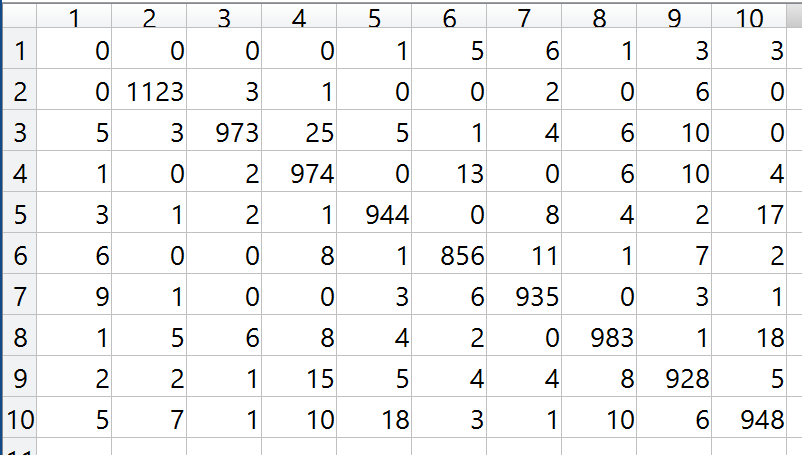
\includegraphics[width=100mm,scale=0.5]{confusionMatrix}


\end{enumerate}

\section{Question 5: Boosting}
We have informally argued that the AdaBoost algorithm uses the weighting mechanism to ``force'' the weak learner to focus on the problematic examples
in the next iteration. In this question we will find some rigorous justification for this argument.
Show that the 0/1 error of $f_t$ w.r.t. the distribution $D_{t+1}$ is exactly 1/2. That is, show that for every $t \in [1, T]$
\[
\sum_{i=1}^m D_{t+1}(\bx_i,y_i) \cdot \boldsymbol{1}[y_i \neq f_t(\bx_i)]=\frac{1}{2}~.
\]
\begin{mdframed}[backgroundcolor=lightgray]
\begin{align}
    D_{t+1}(x,y) &\propto D_{t}(x,y) exp(-\alpha_{t} \cdot y f_{t}(x)) \\
    &= \frac{D_{t}(x,y)}{z} exp(-\alpha_{t} \cdot y f_{t}(x)) \\
    \text{where } \alpha_{t}& = \frac{1}{2} ln\big(\frac{1-\epsilon_{t}}{\epsilon_{t}}\big)
\end{align}
We know that 
\begin{equation}
    y \cdot f_{t}(x) = 
    \begin{cases}
      1, & \text{if correct} \\
      -1, & \text{if wrong}
    \end{cases}
  \end{equation}
Then substituting in the above equation we get,
  \begin{equation}
     D_{t+1}(x,y) = 
    \begin{cases}
       \frac{D_{t}(x,y)}{z} \sqrt{\frac{\epsilon_{t}}{1-\epsilon_{t}}}, & \text{if correct} \\
      \frac{D_{t}(x,y)}{z} \sqrt{\frac{1-\epsilon_{t}}{\epsilon_{t}}}, & \text{if wrong}
    \end{cases}
  \end{equation}
  
Also, all the weights should sum to 1. Thus,
\begin{equation}
\sum_{i=1}^{m}  D_{t+1}(x_i,y_i) = 1
\end{equation}
\begin{equation}
\sqrt{\frac{\epsilon_{t}}{1-\epsilon_{t}}} \frac{1-\epsilon_{t}}{z} + \sqrt{\frac{1-\epsilon_{t}}{\epsilon_{t}}} \frac{\epsilon_{t}}{z} = 1
\end{equation}
\begin{equation}
z = 2 \sqrt{\epsilon_{t} (1-\epsilon_t)}
\end{equation}
Therefore,
  \begin{equation}
     D_{t+1}(x,y) = 
    \begin{cases}
       \frac{D_{t}(x,y)}{2} \frac{1}{1-\epsilon_{t}}, & \text{if correct} \\\\
      \frac{D_{t}(x,y)}{2} \frac{1}{\epsilon_{t}}, & \text{if wrong}
    \end{cases}
  \end{equation}
   0/1 error of $f_t$ w.r.t.  the distribution $D_{t+1} = $
   \begin{align}
       \sum_{i=1}^{m} D_{t+1} (x_i, y_i) \cdot \boldsymbol{1}[y_i \neq f_t(\bx_i)] &=\frac{1}{2 \epsilon_t} \cdot \sum_{i=1}^m D_{t} (x_i, y_i) \cdot \boldsymbol{1}[y_i \neq f_t(\bx_i)]\\
       &= \frac{1}{2 \epsilon_t} \epsilon_t\\
       &= \frac{1}{2}
   \end{align}
   Hence proved.
\end{mdframed}


\section{PCA via Successive Deflation}

Suppose we have a set of $m$ data points $\bx_1, \ldots, \bx_n$, where each $\bx_i$ is represented as a $d$-dimensional column vector. 

Let $\bX = [ \bx_1  \cdots   \bx_m]$ be the $(d \times m)$ matrix where column $i$ is equal to $\bx_i$. Define $C = \frac{1}{m} \bX \bX^\top$ to be the covariance matrix of $\bX$, where $c_{ij} = \sum_{l=1}^{m} \bx_{il} \bx_{jl} = covar(i,j)$.

Next, order the eigenvectors of $C$ by their eigenvalues (largest first), and let $\bv_1, \bv_2, \ldots, \bv_k$ be the first $k$ eigenvectors. These satisfy
\[ 
\bv_i^\top \bv_j =
\begin{cases}
  0 & \mbox{if } i \neq j \\
  1 & \mbox{if } i = j
\end{cases}
\]

$\bv_1$ is the first principal eigenvector of $\bC$ (the eigenvector with the largest eigenvalue), and as such satisfies $\bC \bv_1 = \lambda_1 \bv_1$. Now define $\tilde \bx_i$ as the orthogonal projection of $\bx_i$ onto the space orthogonal to $\bv_1$:
\[
\tilde \bx_i = (\bI - \bv_1 \bv_1^\top) \bx_i~.
\]

Finally, define $\tilde \bX = [\tilde \bx_1  \cdots  \tilde \bx_n]$ as the \textbf{deflated matrix} of rank  $d-1$, which is obtained by removing from the $d$-dimensional data the component that lies in the direction of the first principal eigenvector:
\[
\tilde \bX = (\bI - \bv_1 \bv_1^\top) \bX~.
\]

\subsection{Question 6}
\begin{enumerate}[label=(\alph*)]
\item Show that the covariance of the deflated matrix,
\[
\tilde C  = \frac{1}{m} \tilde \bX \tilde \bX^\top
\]
is given by 
\[
\tilde C = \frac{1}{m} \bX \bX^\top - \lambda_1 \bv_1 \bv_1^\top
\]

\emph{(Hint: Some useful facts: $(I - \bv_1 \bv_1^\top)$ is symmetric, $\bX \bX^\top \bv_1 = m \lambda_1 \bv_1$, and $\bv_1^\top \bv_1 = 1$. Also, for any matrices $A$ and $B$, $(AB)^\top = B^\top A^\top$.)}

\textbf{SOLUTION}
\begin{mdframed}[backgroundcolor=lightgray]
We have:\\\\
 $\tilde C = \frac{1}{m} \tilde \bX \tilde \bX^\top = \frac{1}{m}((I - v_1 v_1^T) \bX ((I - v_1 v_1^T) \bX)^{T})$ \\

(because $(AB)^T = B^TA^T$ and $(I - v_1 v_1^T)$ is symmetric)
\begin{align*}
\tilde C  &= \frac{1}{m} (I - v_1 v_1^T)XX^T(I - v_1 v_1^T)\\
\tilde C  &= \frac{1}{m} (XX^T - v_1 v_1^TXX^T -XX^Tv_1 v_1^T + v_1 v_1^TXX^Tv_1 v_1^T)
\end{align*}

We know that $XX^Tv_1 = m\lambda_1v_1 \Rightarrow (XX^Tv_1)^T = (m\lambda_1v_1)^T \Rightarrow v_1^TXX^T = m\lambda_1v_1^T$. So, 
\begin{align*}
\tilde C  = \frac{1}{m} (XX^T -v_1m\lambda_1v_1^T -m\lambda_1v_1v_1^T + v_1m\lambda_1v_1^Tv_1v_1^T)
\end{align*}

Finally, since $v_1^Tv_1 = 1$
\begin{align*}
\tilde C = \frac{1}{m}XX^T - \lambda_1v_1v_1^T 
\end{align*}
Hence proved.
\end{mdframed}

\item Show that for $j \neq 1$, if $\bv_j$ is a principal eigenvector of $C$ with corresponding eigenvalue $\lambda_j$ (that is, $C \bv_j = \lambda_j \bv_j$), then $\bv_j$ is also a principal eigenvector of $\tilde C$ with the same eigenvalue $\lambda_j$.\\
\textbf{SOLUTION}
\begin{mdframed}[backgroundcolor=lightgray]
\begin{align*}
    \tilde C v_j &= (\frac{1}{m}XX^T - \lambda_1v_1v_1^T)v_j\\
    &= \frac{1}{m}(XX^Tv_j) - \lambda_1v_1v_1^Tv_j\\
    &= \lambda_jv_j - \lambda_1v_1v_1^Tv_j   \texttt{        (since $XX^Tv_j = m\lambda_jv_j$)}
\end{align*}
$\Rightarrow \tilde C v_j = \lambda_jv_j$ (since $v_1^Tv_j = 0$ for $j \neq 1$) \\ and for $j=1$,\\ 
$ \tilde C v_1 = \lambda_1v_1 - \lambda_1v_1v_1^Tv_1 = \lambda_1 v_1 - \lambda_1 v_1 = 0$ \\\\
Hence, for $j \neq 1$, $v_j$ is also a principle eigenvector of $\tilde C$ with same eigenvalue $\lambda_j$. \textbf{Also, $v_1$ is an eigenvector of $\tilde C$ with eigenvalue 0.}
\end{mdframed}

\item Let $\bu$ be the first principal eigenvector of $\tilde C$. Explain why $\bu = \bv_2$. (You may assume $\bu$ is unit norm.)\\
\textbf{SOLUTION}
\begin{mdframed}[backgroundcolor=lightgray]
Since $v_1, v_2, \ldots v_k$ are the first $k$ eigenvectors with largest eigenvalues of $C$, i.e., the principal basis vectors, therefore
\begin{equation*}
\lambda_1 \ge \lambda_2 \ge \ldots \ge \lambda_k
\end{equation*}
From part (b), we know that for $\tilde C$, the principle eigenvectors $v_j$ have eigenvalues $(0,\lambda_2,\lambda_3, \ldots, \lambda_k)$. Since $\lambda_2$ is the largest eigenvalue of $\tilde C$, $v_2$ is the first principle eigenvector of $\tilde C$.\\\\
Hence $\bu = \bv_2$, where $\bu$ be the first principal eigenvector of $\tilde C$.
\end{mdframed}

\item Suppose we have a simple method $f$ for finding the leading eigenvector and eigenvalue of a positive-definite matrix, denoted by
$[\lambda, \bu] = f(C)$. Write some pseudocode for finding the first $k$ principal basis vectors of $\bX$ that only uses the special $f$ function
and simple vector arithmetic.

\emph{(Hint: This should be a simple iterative routine that takes only a few lines to write. The input is $C, k$, and the function $f$, the output
should be $\bv_j$ and $\lambda_j$ for $j \in 1,\cdots, k$)}

\begin{mdframed}[backgroundcolor=lightgray]
\textbf{Pseudocode for finding the first $k$ principal eigenvectors of $X$:}\\
\begin{lstlisting}
function [lambda_list, v_list] = findEigenVectors(k,C,f):
	lambda_list = []
	v_list = []
	for i in range(k):
		lambda, v = f(C)
		C = C - lambda * v * transpose(v)
		lambda_list.append(lambda)
		v_list.append(v)
	return lambda_list, v_list
\end{lstlisting}
\end{mdframed}

\end{enumerate}


\section{Clustering with $k$-means}

In class we discussed the $k$-means clustering algorithm. Your programming assignment this time is to implement the $k$-means algorithm on digit data. 

The goal of clustering can be thought of as minimizing the variation within groups. A good clustering model has low sum of squares within each group. 

We define the sum of squares in the traditional way. Let $\bC_k$ be the $k^{th}$ cluster and let $\bmu_k$ be the mean of the observations in cluster
$\bC_k$. Then the within group sum of squares for cluster $\bC_k$ is defined as:
\[
SS(k) = \sum_{i\in \bC_k} ||\bx_i - \bmu_k||^2_2~.
\]
Please note that the term $||\bx_i - \bmu_k||_2$ is the euclidean distance between
$\bx_i$ and $\bmu_k$.
If there are $K$ clusters in total then the ``total within group sum of squares" is just the sum of all $K$ of these individual $SS(k)$ terms.

The $k$-Means algorithm is a heuristic to minimize the above objective function.


\subsection{The $k$-Means algorithm}

\begin{enumerate}
\item Select $k$ starting centers that are points from your data set. 
\item Assign each data point to the cluster associated with the nearest of the $k$ center points.
\item Re-calculate the centers as the mean vector of each cluster from (2).
\item Repeat steps (2) and (3) until convergence or the limit on the number of iterations is met.
\end{enumerate}

Define convergence as no change in label assignment from one step to another \textbf{or} you have iterated 100 times (whichever comes first). Please count your iterations as follows: after 100 iterations, you should have assigned the points 100 times. 


\subsection{Question 7}

\begin{enumerate}[label=(\alph*)]
\item Implement the $k$-means algorithm as described above. The prototype should be 
\begin{verbatim}
M = kmeans(X, k, T)
\end{verbatim}
where \texttt{X} is the input matrix and \texttt{k} the number of clusters, \texttt{T} the maximum number of iterations to use, and \texttt{M} is the matrix containing the centers.
\begin{minted}[frame=single,framesep=10pt]{matlab}
% Kmeans algorithm.
% X = Xtrain
% k = number of clusters to form
% T = number of iterations
function [M] = kmeans(X, k, T)
    nSamples = size(X,1);
    nFtrs = size(X,2);
    
    % intialize centroids
    centroids = zeros(k, nFtrs);
    randomCentroids = randperm(size(X,1));
    centroids = X(randomCentroids(1:k), :);
    
    for i=1:T
        % find closest centroid
        closestCentroidID = zeros(nSamples,1);
        for j=1:nSamples
            kth = 1;
            minDist = sum(X(j,:) - centroids(kth, :)).^2;
            for m = 2:k
                dist = sum(X(j,:) - centroids(m, :)).^2;
                if(dist < minDist)
                    minDist = dist;
                    kth = m;
                end
            end
            closestCentroidID(j) = kth;
        end
        
        % recompute centroids
        newCentroids = zeros(k, nFtrs);
        for j=1:k
            xj = X(closestCentroidID==j, :);
            count = size(xj, 1);
            newCentroids(j,:) = (1/count) * sum(xj);    
        end
        centroids = newCentroids;
            
    end
    M = centroids;
end
\end{minted}

\item Run the $k$-means algorithm on the training data of MNIST. A plot of the values of the total within group sum of squares for $k = 2$, $k=4$, $k=6$, $k=8$, $k=10$, $k=12$, and $k=14$. Start your centers with the first $k$ points in the dataset.\\
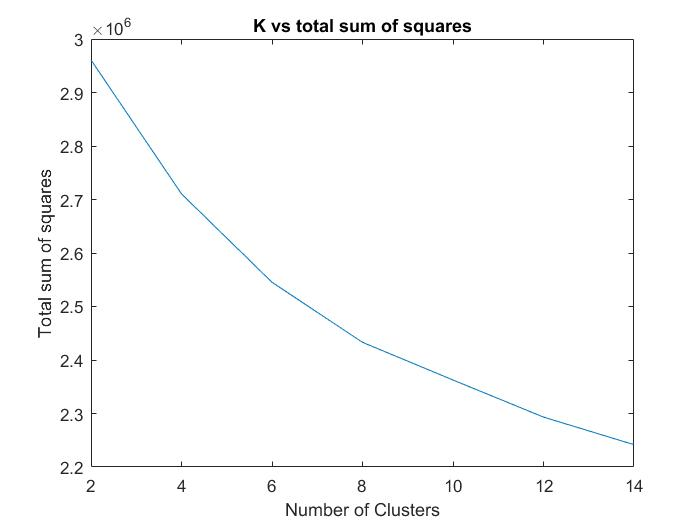
\includegraphics[width=150mm,scale=0.5]{sum_square_3}

\item Let's try to understand how good is $k$-means in recovering the clusters corresponding to the classes. We will use the \emph{cluster purity} as a measure of success. It is defined as 
\[
Purity = \frac{1}{m} \sum_{i=1}^k \max_t |\{j \in C_i \text{ and } y_j=t \}|~.
\]
In words, we associate to each cluster the label corresponding to the class with the majority of the points in the cluster. Hence, having associated a label to each cluster, we can count how many points are correctly classified. Note that the purity can only be calculated in retrospect using the labels associated to each sample, that were unknown during the clustering process.
Plot how the purity change with $k = 2$, $k=4$, $k=6$, $k=8$, $k=10$, $k=12$, and $k=14$.\\
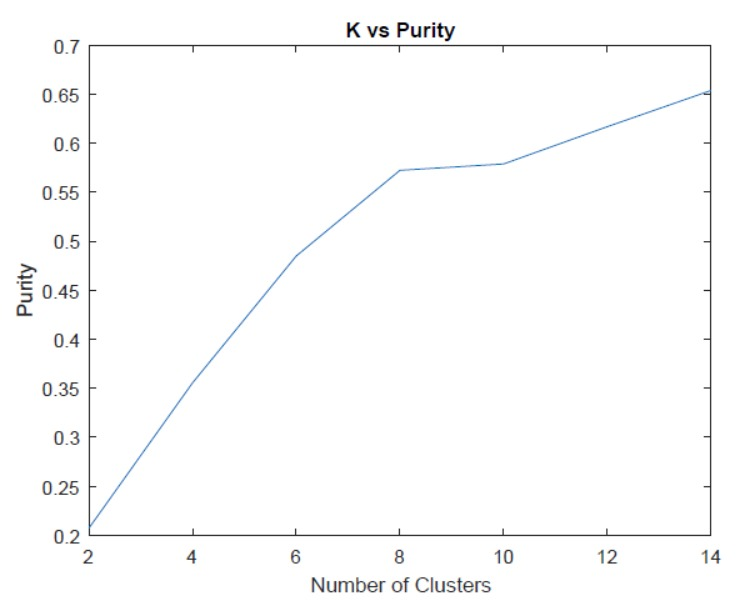
\includegraphics[width=150mm,scale=0.5]{purity_3}
\end{enumerate}

For the last two items, you should run $k$-means algorithm 10 times and average the results. For each question, submit a single plot, which is the average of the runs.


\section{Manual calculation of one round of EM for a Mixture of Gaussians}

In this question we consider clustering 1D data with a mixture of 2 Gaussians using the EM algorithm. You are given the 1-D data points $x = [1 \,\,\, 10 \,\,\, 20]$. 

\subsection*{Question 8}
\textbf{M step.} Suppose the output of the E step is the following matrix:

\[ Q = \left( \begin{array}{cc}
1 & 0 \\
0.4 & 0.6 \\
0 & 1 \end{array} \right)\] 

where entry $Q_{i,c}$ is the probability of observation $x_i$ belonging to cluster $c$. You just have to compute the M step. You may state the equations for maximum likelihood estimates of these quantities without proof; you just have to apply the equations to this data set. You may leave your answer in fractional form.

\begin{enumerate}[label=(\alph*)]
\item Write down the likelihood function you are trying to optimize.
\begin{mdframed}[backgroundcolor=lightgray]
\begin{equation}
Q(\theta, \theta^{(t-1)}) = \sum_{i}{\sum_{c}{Q_{ic}log(\pi_{c})}}  + \sum_{i}{\sum_{c}{Q_{ic}log(p(x_i|\theta_c))}} 
\end{equation}
If the log-liklihod or the parameters converge, we stop else repeat EM.
\end{mdframed}

\item After performing the M step for the mixing weights $\pi_1, \pi_2$, what are the new values?
\begin{mdframed}[backgroundcolor=lightgray]
For any mixture model mixing weights are given by,
\begin{equation}
\pi_c = \frac{1}{N}\sum_i{Q_{ic}} = \frac{Q_c}{N}
\end{equation}
Hence,
\begin{equation}
\pi_1 = \frac{1}{3}(1+0.4+0) = \frac{1.4}{3} = \frac{7}{15} 
\end{equation}
\begin{equation}
\pi_2 = \frac{1}{3}(0+0.6+1) = \frac{1.6}{3} = \frac{8}{15} 
\end{equation}
\end{mdframed}
\item After performing the M step for the means $\mu_1$ and $\mu_2$, what are the new values?
\begin{mdframed}[backgroundcolor=lightgray]
For a Gaussian mixture model, mean is given by,
\begin{equation}
\mu_c = \frac{\sum_i{Q_{ic}x_i}}{Q_c}
\end{equation}
Given 1-D data points x= [1  10  20] and probability matrix Q, we get,
\begin{equation}
\mu_1 = \frac{1*1 + 0.4*10 + 0*20}{1 + 0.4 + 0} = \frac{5}{1.4} = \frac{25}{7}
\end{equation}
\begin{equation}
\mu_2 = \frac{0*1 + 0.6*10 + 1*20}{1 + 0.6 + 0} = \frac{26}{1.6} = \frac{65}{4}
\end{equation}
\end{mdframed}

\item After performing the M step for the standard deviations $\sigma_1$ and $\sigma_2$, what are the new values?
\begin{mdframed}[backgroundcolor=lightgray]
For a Gaussian mixture model, variance is given by,
\begin{equation}
\Sigma_c = \frac{\sum_i{(Q_{ic})(x_i-\mu_c)(x_i - \mu_c)^T}}{Q_c}
\end{equation}
and standard deviation $\sigma$ is given by,
\begin{equation}
\sigma_c = \sqrt{\Sigma_c}
\end{equation}
Substituting 1D data point x = [1 10 20] and probability matrix Q, we get,
\begin{equation}
\Sigma_1 = \frac{1(1-\frac{25}{7})^2 + 0.4(10-\frac{25}{7})^2 + 0(20-\frac{25}{7})^2}{1 + 0.4 + 0} = 16.53 \Rightarrow \sigma_1 = 4.065
\end{equation}

\begin{equation}
\Sigma_2 = \frac{0(1-\frac{65}{4})^2+0.6(10-\frac{65}{4})^2+ 1(20-\frac{65}{4})^2}{0 + 0.6 + 1} = 23.4375 \Rightarrow \sigma_2 = 4.84 
\end{equation}
\end{mdframed}

\end{enumerate}

\noindent \textbf{E step.} Now suppose the output of the M step is the answer to the previous section. You will compute the subsequent E step.

\begin{enumerate}[label=(\alph*),resume]
\item Write down the formula for the probability of observation $x_i$ belonging to cluster $c$.
\begin{mdframed}[backgroundcolor=lightgray]
The probability of observation $x_i$ belonging to cluster c:
\begin{equation}
Q_{ic} = \frac{\pi_cp(x_i|\theta_c^{(t-1)})}{\sum_{c'}{\pi_{c'}p(x_i|\theta_{c'}^{(t-1)})}} 
\end{equation}
where,
\begin{equation}
p(x_i|\theta_c^{(t-1)}) = \frac{1}{\sigma_c\sqrt{2\pi}}\exp{-\frac{1}{2}\bigg(\frac{x_i - \mu_c}{\sigma_c}\bigg)^2}
\end{equation}
\end{mdframed}

\item After performing the E step, what is the new value of $Q$?
\begin{mdframed}[backgroundcolor=lightgray]
Using the two equations above and plugging in the values from \textbf{M-step}, we get: 
\begin{align*}
p(x_1|\theta_1) &= \frac{1}{4.065\sqrt{2\pi}}\exp{-\frac{1}{2}\bigg(\frac{1 - \frac{25}{7}}{4.065}\bigg)^2} = 0.0803\\
p(x_1|\theta_2) &= \frac{1}{4.84\sqrt{2\pi}}\exp{-\frac{1}{2}(\frac{1 - \frac{65}{4}}{4.84})^2} = 0.000575\\
p(x_2|\theta_1) &= \frac{1}{4.065\sqrt{2\pi}}\exp{-\frac{1}{2}(\frac{10 - \frac{25}{7}}{4.065})^2} = 0.028\\
p(x_2|\theta_2) &= \frac{1}{4.84\sqrt{2\pi}}\exp{-\frac{1}{2}(\frac{10 - \frac{65}{4}}{4.84})^2} = 0.0358\\
p(x_3|\theta_1) &= \frac{1}{4.065\sqrt{2\pi}}\exp{-\frac{1}{2}(\frac{20 - \frac{25}{7}}{4.065})^2} = 0.0000278\\
p(x_3|\theta_2) &= \frac{1}{4.84\sqrt{2\pi}}\exp{-\frac{1}{2}(\frac{20 - \frac{65}{4}}{4.84})^2} = 0.061\\
\end{align*}

Hence, 
\begin{align*}
Q_{11} &= \frac{\frac{7}{15}0.0803}{\frac{7}{15}0.0803 + \frac{8}{15}0.000575} = 0.992\\\\
Q_{12} &= 1 - Q_{11} = 1 - 0.992  = 0.008\\\\
Q_{21} &= \frac{\frac{7}{15}0.028}{\frac{7}{15}0.028 + \frac{8}{15}0.0358} = 0.406\\\\
Q_{22} &= 1 - Q_{21} = 1 - 0.406  = 0.594\\\\
Q_{31} &= \frac{\frac{7}{15}0.0000278}{\frac{7}{15}0.0000278 + \frac{8}{15}0.061} = 0.00039\\\\
Q_{32} &= 1 - Q_{31} = 1 - 0.00039  = 0.99961
\end{align*}

\[ Q_{new} = \left( \begin{array}{cc}
0.992 & 0.008 \\
0.406 & 0.594 \\
0.00039 & 0.99961 \end{array} \right)\] 
\end{mdframed}

\end{enumerate}

{\small
\bibliographystyle{plain}
\bibliography{learning}
}

\end{document} 
